% !TeX root = final-report.tex
\pdfoutput=1

\documentclass[11pt]{article}

\usepackage[]{acl}
\usepackage[T1]{fontenc}
\usepackage[utf8]{inputenc}
\usepackage{algorithm2e}
\usepackage{amsmath}
\usepackage{amssymb}
\usepackage{array}
\usepackage{booktabs}
\usepackage{colortbl}
\usepackage{dsfont}
\usepackage{enumitem}
\usepackage{etoolbox}
\usepackage{float}
\usepackage{graphicx}
\usepackage{hyperref}
\usepackage{inconsolata}
\usepackage{latexsym}
\usepackage{listings}
\usepackage{makecell}
\usepackage{mathrsfs}
\usepackage{microtype}
\usepackage{multirow}
\usepackage{pifont}
\usepackage{relsize}
\usepackage{scalerel}
\usepackage{svg}
\usepackage{tabularx}
\usepackage{times}
\usepackage{url}
\usepackage{xcolor,soul}

\lstset{ 
  backgroundcolor=\color{white},
  basicstyle=\scriptsize\ttfamily,
  breakatwhitespace=false,
  breaklines=true,
  captionpos=b,
  commentstyle=\color{green},
  escapeinside={\%*}{*)},
  extendedchars=false,
  frame=lrtb,
  keepspaces=true,
  keywordstyle=\color{blue},
  language=Python,
  morekeywords={with,as},
  numbers=none,
  numbersep=5pt,
  numberstyle=\tiny\color{gray},
  rulecolor=\color{black},
  showspaces=false,
  showstringspaces=false,
  showtabs=false,
  stringstyle=\color{purple},
  tabsize=4,
  title=\lstname,
  xleftmargin=.2cm,
  xrightmargin=.2cm,
  aboveskip=1.2em,
  belowskip=-1.5 \baselineskip,
  belowcaptionskip=0em,
}

\definecolor{lblue}{HTML}{A6CEE3}
\definecolor{lgreen}{HTML}{B2DF8A}
\definecolor{lred}{HTML}{FB9A99}
\definecolor{lorange}{HTML}{FDBF6F}
\definecolor{mblue}{HTML}{80B1D3}
\definecolor{mgreen}{HTML}{B3DE69}
\definecolor{mred}{HTML}{FB8072}
\definecolor{morange}{HTML}{FDB462}
\definecolor{blue}{HTML}{1F78B4}
\definecolor{green}{HTML}{33A02C}
\definecolor{red}{HTML}{E31A1C}
\definecolor{orange}{HTML}{FF7F00}
\definecolor{dblue}{HTML}{08519C}
\definecolor{dgreen}{HTML}{006D2C}
\definecolor{dorange}{HTML}{EC7014}
\newcommand{\blue}[1]{{\color{blue} #1}}
\newcommand{\green}[1]{{\color{green} #1}}
\newcommand{\red}[1]{{\color{red} #1}}
\newcommand{\orange}[1]{{\color{orange} #1}}
\newcommand{\dblue}[1]{{\color{dblue} #1}}
\newcommand{\dgreen}[1]{{\color{dgreen} #1}}
\newcommand{\dorange}[1]{{\color{dorange} #1}}
\sethlcolor{yellow}

\newcommand{\Tablink}[1]{\hyperref[#1]{Table~\ref*{#1}}}
\newcommand{\Figlink}[1]{\hyperref[#1]{Figure~\ref*{#1}}}

% TODO: add code links
\newif\ifshowcodelinks
\showcodelinksfalse

\newcommand{\codelink}[1]{%
\ifshowcodelinks
[\href{#1}{Code}]%
\fi
}

\title{%
  XCS224U Final Project Report\textsuperscript{*} \\
  
\includegraphics[height=1em]{images/emoji.png}%
  \hspace{0.1em} \textit{Academic Anonymity: Advancing PII Detection in Essays through Longformer}%
}

\author{Jonathan Algar \\
  Lisbon, Portugal \\
  \texttt{\href{mailto:jonathan.algar@gmail.com}{jonathan.algar@gmail.com}}
}

\newcounter{savedfootnote}

% Command to switch to dagger footnotes
\newcommand{\daggerfootnotes}{
    \setcounter{savedfootnote}{\value{footnote}} % Save current footnote number
    \renewcommand{\thefootnote}{\fnsymbol{footnote}}
    \setcounter{footnote}{1} % Start daggers
}

% Command to switch back to numeric footnotes and continue from last saved
\newcommand{\numericfootnotes}{
    \setcounter{footnote}{\value{savedfootnote}} % Restore footnote number
    \renewcommand{\thefootnote}{\arabic{footnote}}
}

\begin{document}

\maketitle
\vspace{-1em}
\begin{center}
\small\textit{\textsuperscript{*}{Updated since submission. \\ Last update: \today}.}
\end{center}

\begin{abstract}

This project concerns the task of detecting Personally Identifiable Information (PII) in a domain-specific text corpus. The experiments in this project use student essays as the domain.

Microsoft's Presidio SDK \cite{Presidio} has established itself as the default choice for industry practitioners for the task of detecting PII, irrespective of the domain (see, for example, \citealt{AzizStraiton2023PIIDetection}). This choice is especially true since Presidio's recent integration with popular \href{https://python.langchain.com/docs/guides/productionization/safety/presidio_data_anonymization/}{practitioner tools such as LangChain}.

This project shows that a Longformer model \cite{abs-2004-05150} fine-tuned on a high-quality, human-annotated, domain-specific dataset yields considerable outperformance in the identification of PII ($F_5 = 0.831$) over the Presidio benchmark ($F_5 = 0.735$).

Furthermore, I show that synthetically generated data can be highly effective in supplementing a train set to bolster overall performance ($F_5 = 0.936$).

The result supports the long-standing conclusion of \citealt{Chen2015ASO} (summarized by \citealt{hathurusinghe-etal-2021-privacy}) that for the training of a robust PII recognizer, a customized domain-specific annotated dataset is needed.

I conclude by discussing potential directions for further research and novel industry applications based on the results of these experiments.

\end{abstract}

\section{Hypothesis}

Microsoft's Presidio SDK \cite{Presidio} has established itself as the default choice for industry practitioners for the task of detecting PII, irrespective of the domain (see, for example, \citealt{AzizStraiton2023PIIDetection}). This choice is especially true since Presidio's recent integration with popular \href{https://python.langchain.com/docs/guides/productionization/safety/presidio_data_anonymization/}{practitioner tools such as LangChain}. The recognition engine uses a combination of techniques to detect PII entities: regular expressions, NER using spaCy, and predefined context words.

I will apply the SDK to the test set of a novel domain-specific dataset: student essays.

I hypothesize that the benchmark will be significantly outperformed, as measured by standard classifier metrics, by a custom model fine-tuned on the train set of a high-quality, human-annotated, domain-specific dataset.

If the primary hypothesis holds, it would add a further data point in support of the conclusion of \citealt{Chen2015ASO} (summarized by \citealt{hathurusinghe-etal-2021-privacy}) that for the training of a robust PII recognizer, a customized domain-specific annotated dataset is needed.

The secondary hypothesis is that the primary hypothesis holds principally because of \textit{in-context PII}, which is highly domain-specific.

\section{Prior literature}

The main problem addressed by the related published papers I assessed is how to use a corpus containing sensitive data for machine learning and downstream NLP tasks while protecting privacy. This is an important problem because:

\begin{itemize}
\item Clinical text, for example, contains a wealth of valuable information that can be used to train machine-learning models for various healthcare applications. However, this data also contains sensitive personal information about patients that must be kept private.
\item Regulations like The Health Insurance Portability and Accountability Act of 1996 (HIPAA) in the United States and General Data Protection Regulation (GDPR) in the European Union place strict requirements on the handling of personal information. De-identification is often necessary for data to be used for research purposes in compliance with these regulations.
\item At the same time, over-zealous de-identification can destroy the utility of the data for machine learning. It is important to advance methods that protect privacy while preserving as much useful information as possible.
\end{itemize}

Since around 2020 the machine learning literature been unanimous in using transformers as the baseline for identifying PII in domain-specific corpora, irrespective of the domain or structure of the underlying text.

The domain of the underlying corpora varies across the related published papers I assessed. For example, while \citealt{hathurusinghe-etal-2021-privacy} and \citealt{vakili-etal-2022-downstream} focus on the medical domain, \citealt{pilan-etal-2022-text} focus on legal cases, and \citealt{vanderplas2022detecting} on code.

\citealt{pilan-etal-2022-text} is the key paper for the intrinsic evaluation of text anonymization methods. The paper presents the Text Anonymization Benchmark (TAB), an annotated corpus and associated set of evaluation metrics designed to assess the performance of text anonymization methods. 

The authors found a Longformer model fine-tuned on the TAB train set achieved superior performance across all the metrics against two baseline methods: Neural NER (RoBERTa)\footnote{\textit{"A neural NER model based on the RoBERTa language model (Liu et al. 2019) and fine-tuned for NER on Ontonotes v5 (Weischedel et al. 2011), as implemented in spaCy."}} and Presidio\footnote{\textit{"We provide evaluation results for Presidio under two configuration settings, namely, the default mode and one in which the detection of organization names (governments, public administration, companies, etc.) is also activated."}}.

\section{Data}

The data used for the experiements in this paper is a corpus of 22,000 academic essays written by students enrolled in a Massive Open Online Course (MOOC) at Vanderbilt University in response to a single question.

This novel data was distributed in the context of a Kaggle competition \cite{pii-detection-removal-from-educational-data}. The publicly distributed version of the dataset skews $70\%$ to the \textit{unannotated} test set versus $30\%$ annotated for train and dev. For the experiment I advance in this project on the publicly distributed version of the data, I will focus on the $30\%$ of annotated essays and split these $6,807$ samples $80\%$ for train, $10\%$ for dev, and $10\%$ test.

The data is distributed as a \texttt{json} \cite{pii-detection-removal-from-educational-data} and contains the following keys for each student essay:

\begin{itemize}
  \label{par:pii_types}
  \item \texttt{document}: An integer ID uniquely identifying the essay.
  \item \texttt{full\_text}: The complete text of the essay as a UTF-8 string. Includes all of the essay's content as it was submitted without modification.
  \item \texttt{tokens}: A list of strings, each representing a tokenized portion of the \texttt{full\_text}. The SpaCy tokenizer \cite{honnibal2020spacy} was used for tokenization.
  \item \texttt{trailing\_whitespace}: A list of boolean values corresponding to each token in the \texttt{tokens} list. Each boolean indicates whether the token is followed by whitespace in the \texttt{full\_text}.
  \item \texttt{labels}: A list of labels in the BIO (Beginning, Inner, Outer) format, corresponding to each token in the \texttt{tokens} list. A label with a prefix of \texttt{B-} indicates the beginning of a PII entity, \texttt{I-} signifies a continuation of a PII entity, and \texttt{O} indicates the token is not considered PII. This labeling schema facilitates precise identification and categorization of PII within the essays. See \Figlink{fig:label_visualization} for a visual example of the labeling of the top part of one essay's \texttt{full\_text}. 
\end{itemize}

The essays contain the following types of PII entities:

\begin{itemize}
  \item \texttt{NAME\_STUDENT}: The full or partial name of a student. This type includes only the names of students and excludes names of instructors, authors, or any other individuals.
  \item \texttt{EMAIL}: The email address associated with a student.
  \item \texttt{USERNAME}: Any username a student uses which could provide hints to their identity or activities.
  \item \texttt{ID\_NUM}: A unique number or sequence of characters assigned to a student, such as a student ID or social security number, that can be used for identification.
  \item \texttt{PHONE\_NUM}: A contact phone number belonging to a student.
  \item \texttt{URL\_PERSONAL}: A URL that is personally associated with a student. Includes blogs, portfolios, or profiles.
  \item \texttt{STREET\_ADDRESS}: The full or partial physical address of a student. This includes any information that could be used to physically locate a student.
\end{itemize}

\begin{figure*}[t]
  \centering
  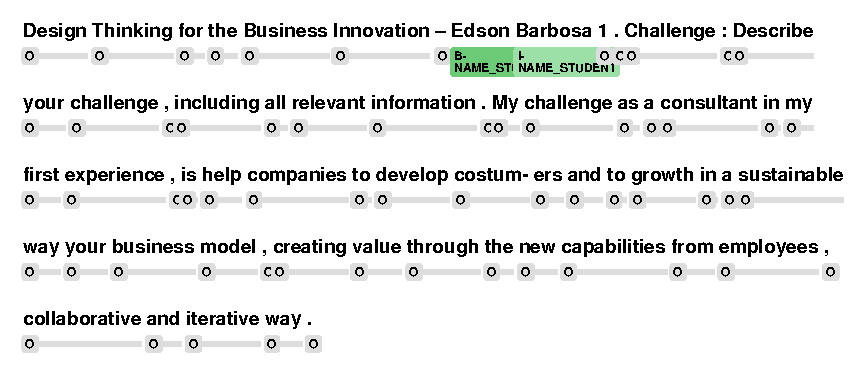
\includegraphics[width=1.0\linewidth]{images/label_visualization.pdf}
  \caption{Using \texttt{displaCy} to visualize the BIO labels associated with the tokens of the first two sentences of a randomly selected essay containing PII in the original train set.}
  \label{fig:label_visualization}
\end{figure*}

\subsection{Analysis of original train set}

\Tablink{tab:pii_distribution_original_train_set} shows only a minority of essays in the originally constructed train set contain any PII.

\begin{table}[h!]
  \centering
  \caption{Distribution of essays with and without PII in the original train set.}
  \label{tab:pii_distribution_original_train_set}
  \begin{tabular}{lrl}
  \toprule
            Category &  Count & Percentage \\
  \midrule
     Essays with PII &    763 &        14\% \\
  Essays without PII &   4682 &        86\% \\
        Total essays &   5445 &       100\% \\
  \bottomrule
  \end{tabular}
\end{table}

And \Figlink{fig:label_distribution_original_train_set} shows the distribution of PII is heavily skewed to student names. Indeed, for several BIO labels, there are very few examples.

\begin{figure}[H]
  \centering
  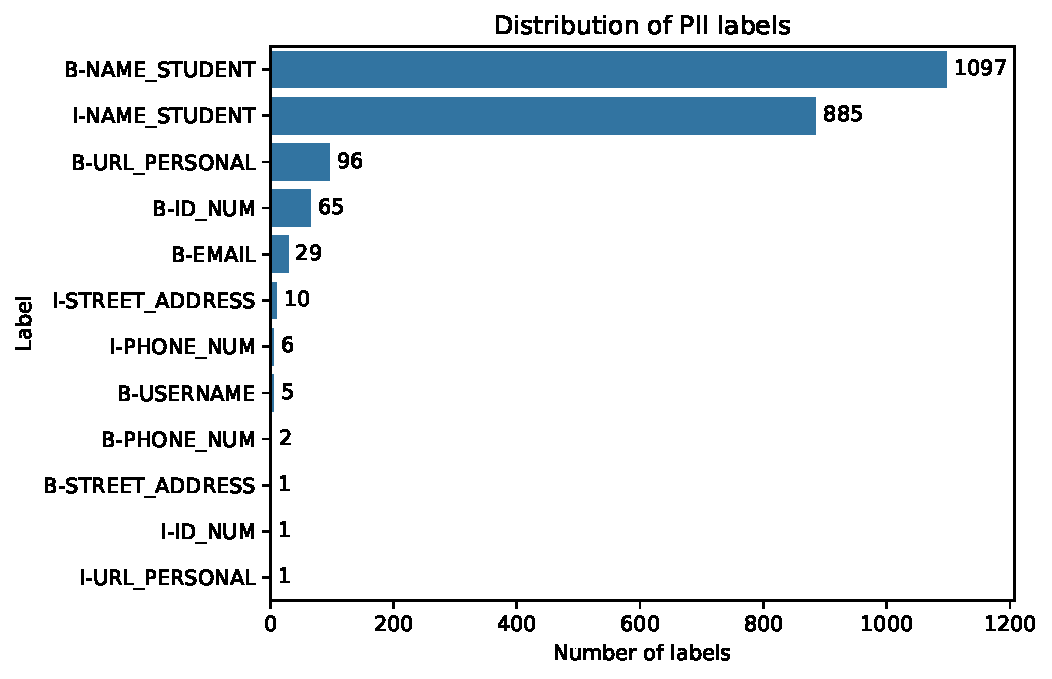
\includegraphics[width=\columnwidth]{images/label_distribution.pdf}
  \caption{Original train set.}
  \label{fig:label_distribution_original_train_set}
\end{figure}

\subsection{Synthetic data}

To address the limited number of examples of a subset of the BIO labels in the original train set, I augment it with 1000 synthetically generated labeled essays.

To achieve this, I first use the Faker library \cite{Faraglia2023Faker} to generate 1000 sets of PII data. An example set:

\begin{lstlisting}
{
  'ID_NUM': '739916633Gmhl3hvcXqDgCIug',
  'NAME_STUDENT': 'Bryan Evans',
  'EMAIL': 'bryan.evans@gonzalez.com',
  'USERNAME': 'bryan.evans5',
  'PHONE_NUM': '+1-876-799-4028x1242',
  'URL_PERSONAL': 'https://youtube.com/c/bryan.evans5',
  'STREET_ADDRESS': '584 Patrick Hollow Apt. 760 North Keith, DE 20952'
}
\end{lstlisting}

Based on the observed patterns of PII in the essays in the train set, I constructed two prompts.

\verb|PROMPT_1|:

\begin{lstlisting}
  {
    "role": "system",
    "content": "You are a student tasked with writing an essay on how you applied a specific design thinking tool to address a challenge or problem in your life. In addition, you will be given a JSON containing your personal information: ID_NUM, NAME_STUDENT, EMAIL, USERNAME, PHONE_NUM, URL_PERSONAL, STREET_ADDRESS. Include all this information in the essay in a suitable format at the beginning of the essay."
  },
  {
    "role": "user",
    "content": "Your personal information: " + str(pii_set)
  }
\end{lstlisting}

\verb|PROMPT_2|:

\begin{lstlisting}
  {
    "role": "system",
    "content": "You are a student tasked with writing an essay on how you applied a specific design thinking tool to address a challenge or problem in your life. In addition, you will be given a JSON containing your personal information: ID_NUM, NAME_STUDENT, EMAIL, USERNAME, PHONE_NUM, URL_PERSONAL, STREET_ADDRESS. Weave all this personal information into the essay."
  },
  {
    "role": "user",
    "content": "Your personal information: " + str(pii_set)
  }
\end{lstlisting}

50\% of the set of generated PII data were allocated to \verb|PROMPT_1| and 50\% to \verb|PROMPT_2|. I generated the essays using OpenAI's \verb|gpt-3.5-turbo-0125| model with \verb|temperature=0.7|. Post-processing was then done to construct a dataset congruent with the original train set. This included tokenizing the essays using the SpaCy tokenizer \cite{honnibal2020spacy}, generating the \verb|trailing_whitespace| boolean list, and assigning the appropriate BIO labels.

\subsubsection{Analysis of synthetic data}

\begin{table}[h!]
  \centering
  \caption{
    Distribution of essays with and without PII in the generated synthetic dataset.}
  \label{tab:pii_distribution_synth}
  \begin{tabular}{lrl}
  \toprule
            Category &  Count & Percentage \\
  \midrule
     Essays with PII &    948 &      94.8\% \\
  Essays without PII &     52 &       5.2\% \\
        Total essays &   1000 &       100\% \\
  \bottomrule
  \end{tabular}
\end{table}

And \Figlink{fig:label_distribution_synth} shows a far more balanced distribution of PII labels relative to the original train set.

\begin{figure}[h!]
  \centering
  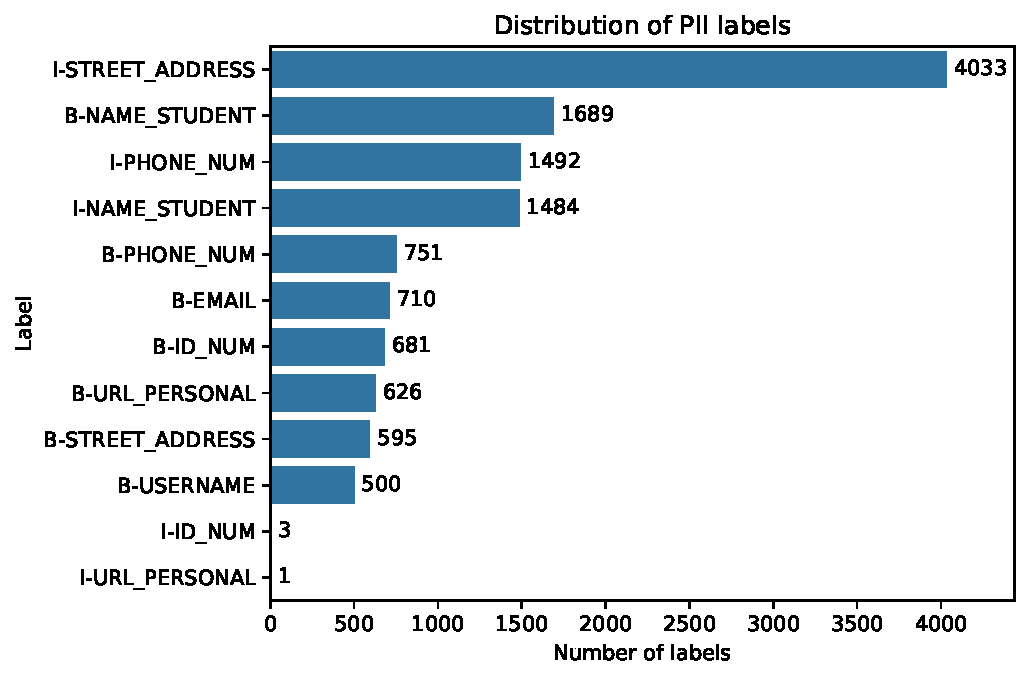
\includegraphics[width=\columnwidth]{images/label_distribution_synth.pdf}
  \caption{Train set with synthetic data.}
  \label{fig:label_distribution_synth}
\end{figure}

\section{Model}

\subsection{High-level overview}
The Longformer \cite{abs-2004-05150} is a BERT-style transformer designed to efficiently process long documents using a combination of sliding window local attention and global attention. It is built on top of the RoBERTa checkpoint and was pre-trained on long documents using a masked language modeling objective. \citealt{pilan-etal-2022-text} showed it is a strong base model to use for the task of identifying PII.

The full architecture of the model used for this paper's experiments:

\begin{enumerate}
  \setcounter{enumi}{-1}
  \item \href{https://huggingface.co/allenai/longformer-base-4096}{\texttt{allenai/longformer-base-4096}} to process the tokenized input essays and produce contextualized token representations.
  \item A bidirectional long short-term memory (LSTM) layer to further refine the token representations and capture sequential dependencies.
  \item A linear output layer to project the LSTM hidden states onto the space of BIO labels.
  \item A softmax activation function applied to the output layer to obtain probability distributions over the BIO labels for each token.
\end{enumerate}

\begin{lstlisting}
INFO:lightning.pytorch.callbacks.model_summary:
  | Name               | Type            | Params
-------------------------------------------------
0 | transformers_model | LongformerModel | 148 M 
1 | head               | LSTMHead        | 3.5 M 
2 | output             | Linear          | 10.0 K
3 | loss_function      | CrossEntropyLoss| 0     
-------------------------------------------------
152 M     Trainable params
0         Non-trainable params
152 M     Total params
608.858   Total estimated model params size (MB)
\end{lstlisting}

The model was fine-tuned on two datasets independently: (1) the original train set and (2) the original train set augmented with the synthetically generated data. The objective was to minimize the cross-entropy loss between the predicted BIO label probabilities and the human-annotated gold BIO labels. To address class imbalance, essays without PII were downsampled during training.

During training the model was optimized using the \texttt{AdamW} optimizer with a learning rate of $1 \times 10^{-5}$ and a cosine learning rate scheduler. Training was for a maximum of four epochs with five-fold stratified cross-validation.

\subsection{Mathematical summary}
Let $\mathbf{x} = (x_1, \ldots, x_n)$ be the input sequence of tokens for a given student essay. The Longformer computes a contextualized representation $\mathbf{h} = (h_1, \ldots, h_n)$, where $h_i \in \mathbb{R}^d$ ($d=768$) is the hidden state corresponding to token $x_i$. The Longformer uses a combination of local and global attention to efficiently process long sequences:

\begin{equation*}
\mathbf{h}^{(l)} = \texttt{LocalAttn}(\mathbf{h}^{(l-1)}, \mathbf{W}_Q^{(l)}, \mathbf{W}_K^{(l)}, \mathbf{W}_V^{(l)})
\end{equation*}
\begin{equation*}
\mathbf{h}^{(g)} = \texttt{GlobalAttn}(\mathbf{h}^{(l)}, \mathbf{W}_Q^{(g)}, \mathbf{W}_K^{(g)}, \mathbf{W}_V^{(g)})
\end{equation*}

where $\mathbf{W}_Q^{(l)}, \mathbf{W}_K^{(l)}, \mathbf{W}_V^{(l)}, \mathbf{W}_Q^{(g)}, \mathbf{W}_K^{(g)}, \mathbf{W}_V^{(g)}$ are learnable parameters for the local and global attention mechanisms, respectively. The local attention is computed within a fixed-size window around each token, while the global attention allows a subset of tokens to attend to all other tokens in the sequence.

The LSTM layer further processes the hidden states to produce refined representations $\mathbf{r} = (r_1, \ldots, r_n)$. The final linear layer maps the refined representations to the BIO label probabilities:

\begin{equation*}
\mathbf{p}_i = \text{softmax}(\mathbf{W}r_i + \mathbf{b})
\end{equation*}

where $\mathbf{W} \in \mathbb{R}^{k \times d}$ and $\mathbf{b} \in \mathbb{R}^k$ are learnable parameters. $k=13$ is the number of BIO labels.

The model is trained to minimize the standard cross-entropy loss:

\begin{equation*}
\mathcal{L} = -\frac{1}{n} \sum_{i=1}^n \sum_{j=1}^k y_{ij} \log p_{ij}
\end{equation*}

where $y_{ij}$ is the true BIO label for token $x_i$ and BIO label $j$, and $p_{ij}$ is the predicted probability of token $x_i$ having BIO label $j$.


\subsection{Notes on Longformer and PII}

The Longerformer's local attention mechanism is confined to small windows surrounding each token. By attending to the local context, the model remains responsive to the syntactic structure of the text—essential for accurately identifying PII entities such as student names, often contextually dependent on nearby words.

On the other hand, global attention allows select tokens to attend to the entire text, enabling the model to integrate broader narrative contexts. This is particularly useful in essays where references to PII can be subtly woven into the text or contextualized across different sections of the same essay. By maintaining an awareness of the entire essay, the Longformer can better understand the relevance and implications of specific tokens, enhancing its ability to discern PII from similarly structured non-PII text.

The combination of local and global attention mechanisms allows the Longformer to effectively navigate the dual challenges of length and complexity in student essays. By focusing on local relevance while simultaneously integrating global context, the model strikes a balance between depth of focus and breadth of understanding. This makes it particularly well-suited for the nuanced task of detecting PII in essays, where the context and narrative structure of the essays play a significant role in identifying sensitive information.

\subsection{Training runs}

Charts generated by Weights \& Biases \cite{wandb}.

\begin{figure}[H]
  \centering
  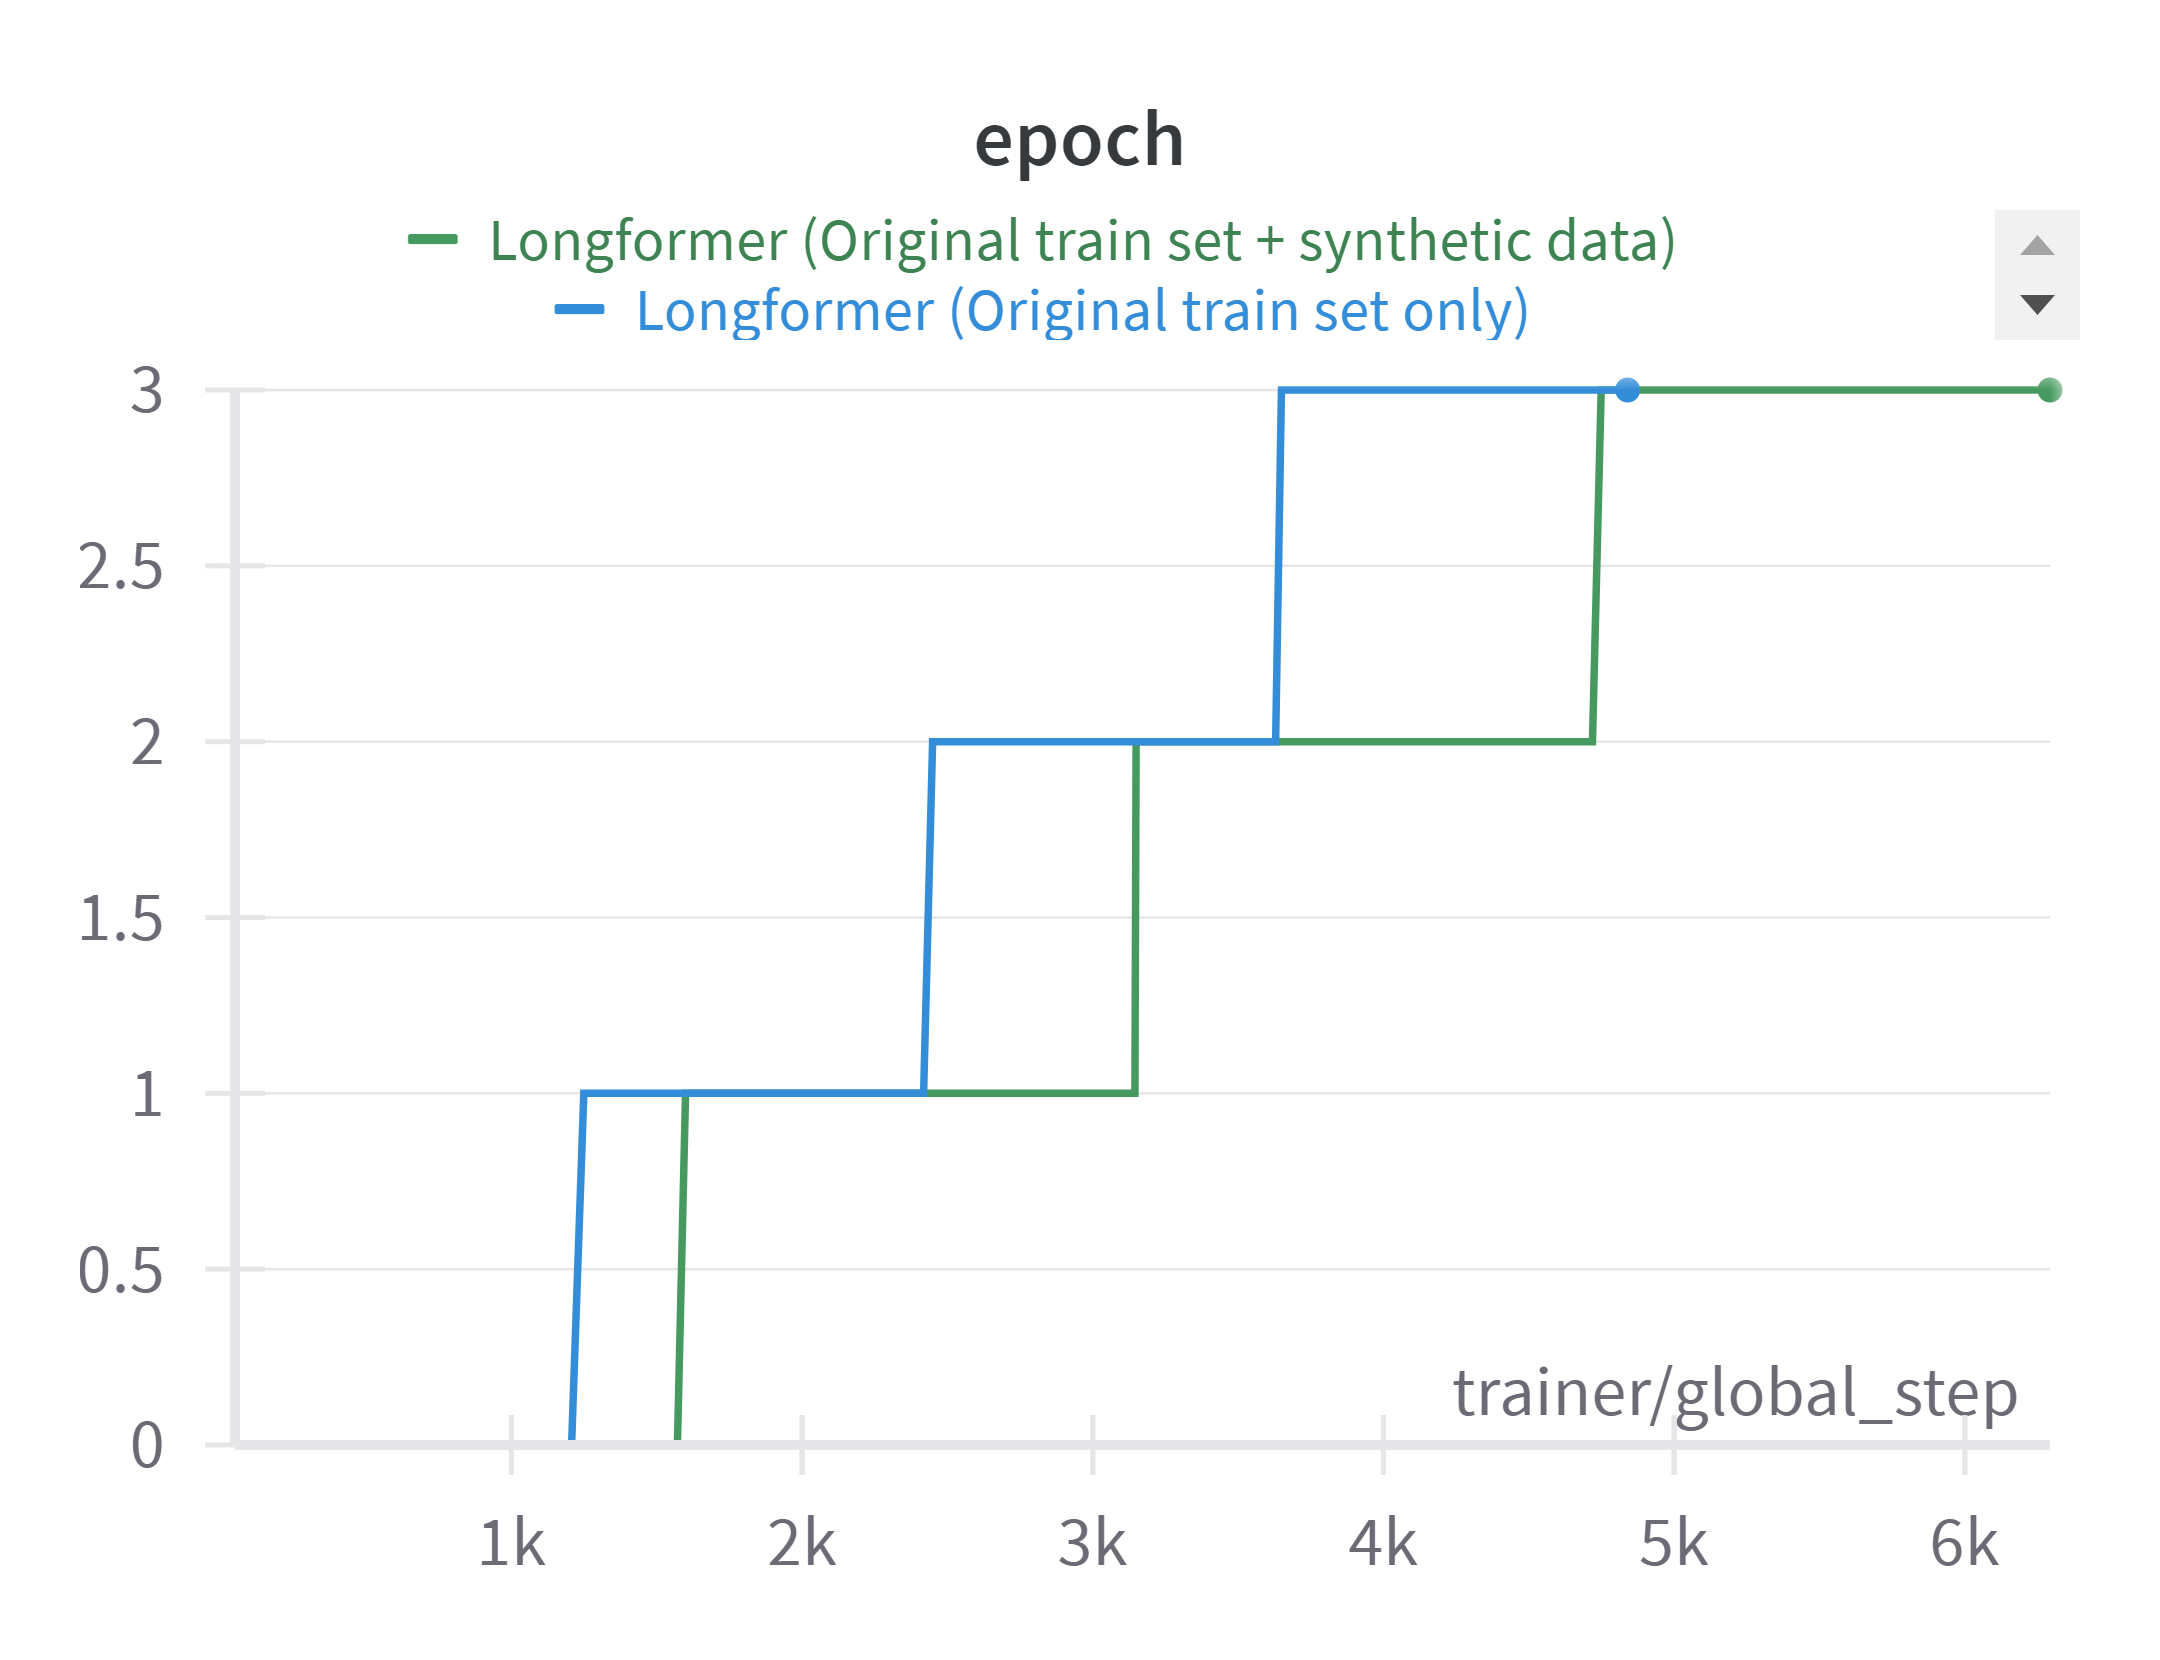
\includegraphics[width=\columnwidth]{images/epochs.png}
  \label{fig:epochs}
\end{figure}

\begin{figure}[H]
  \centering
  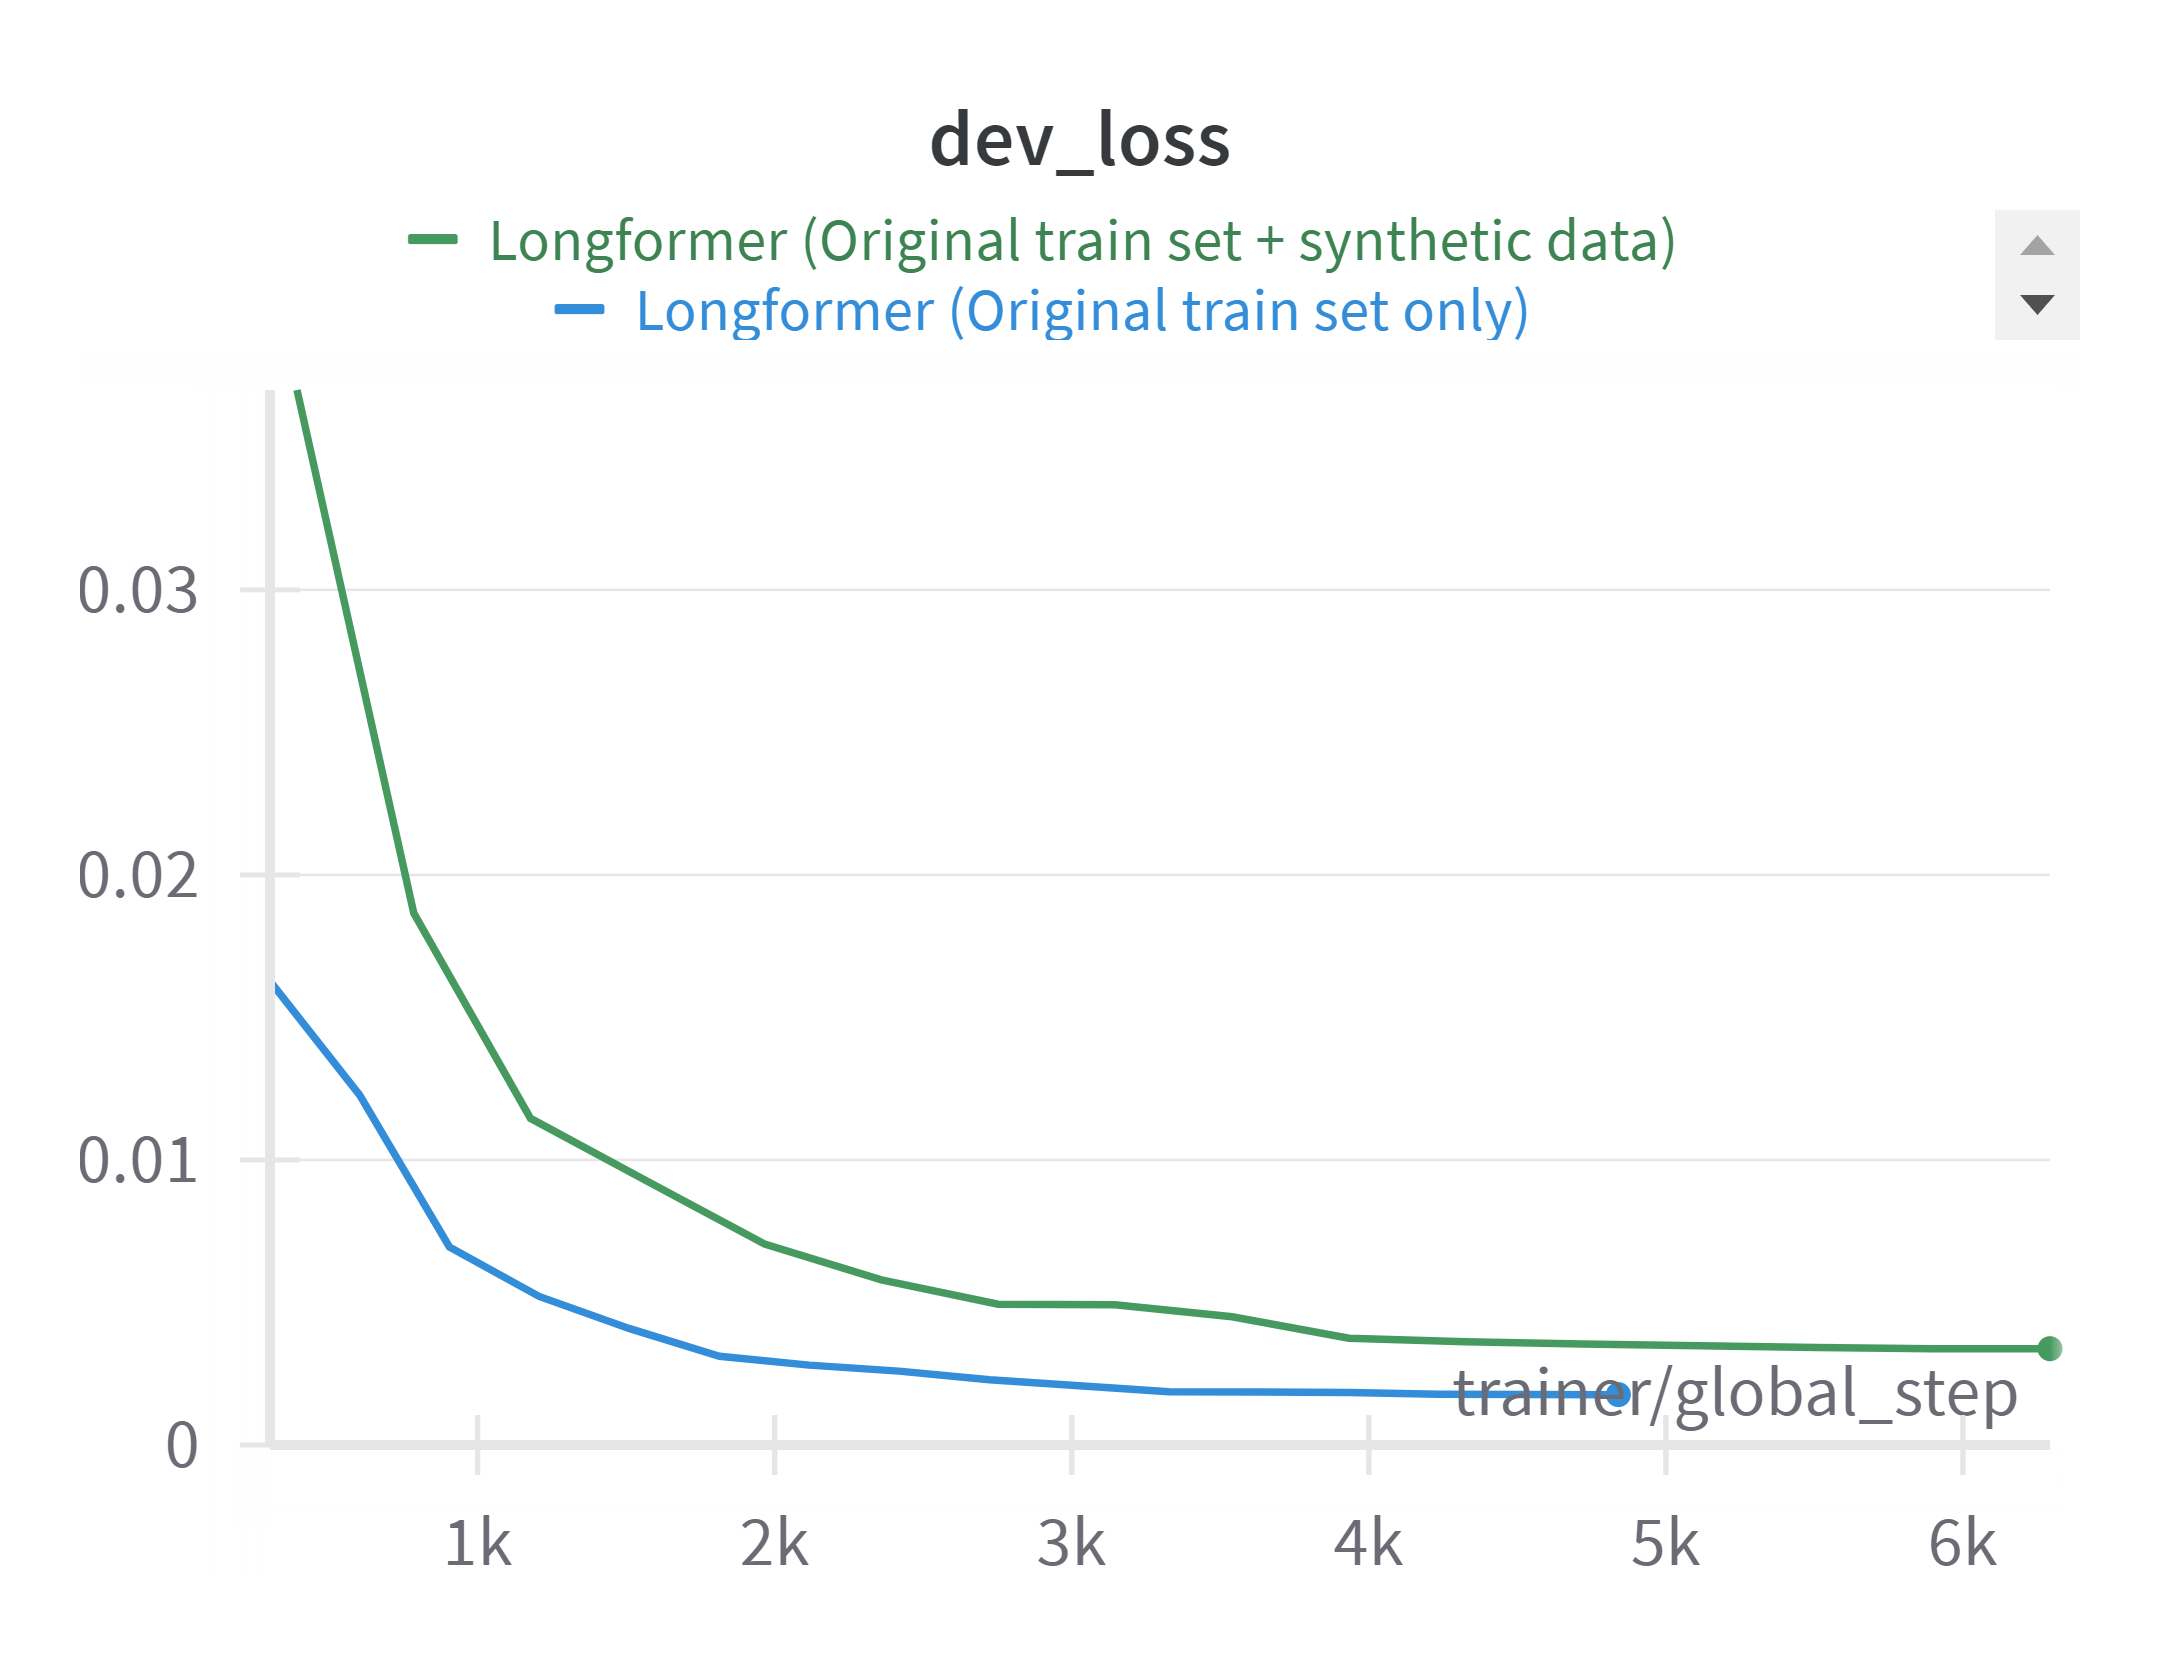
\includegraphics[width=\columnwidth]{images/dev_loss.png}
  \label{fig:dev_loss}
\end{figure}

\begin{figure}[H]
  \centering
  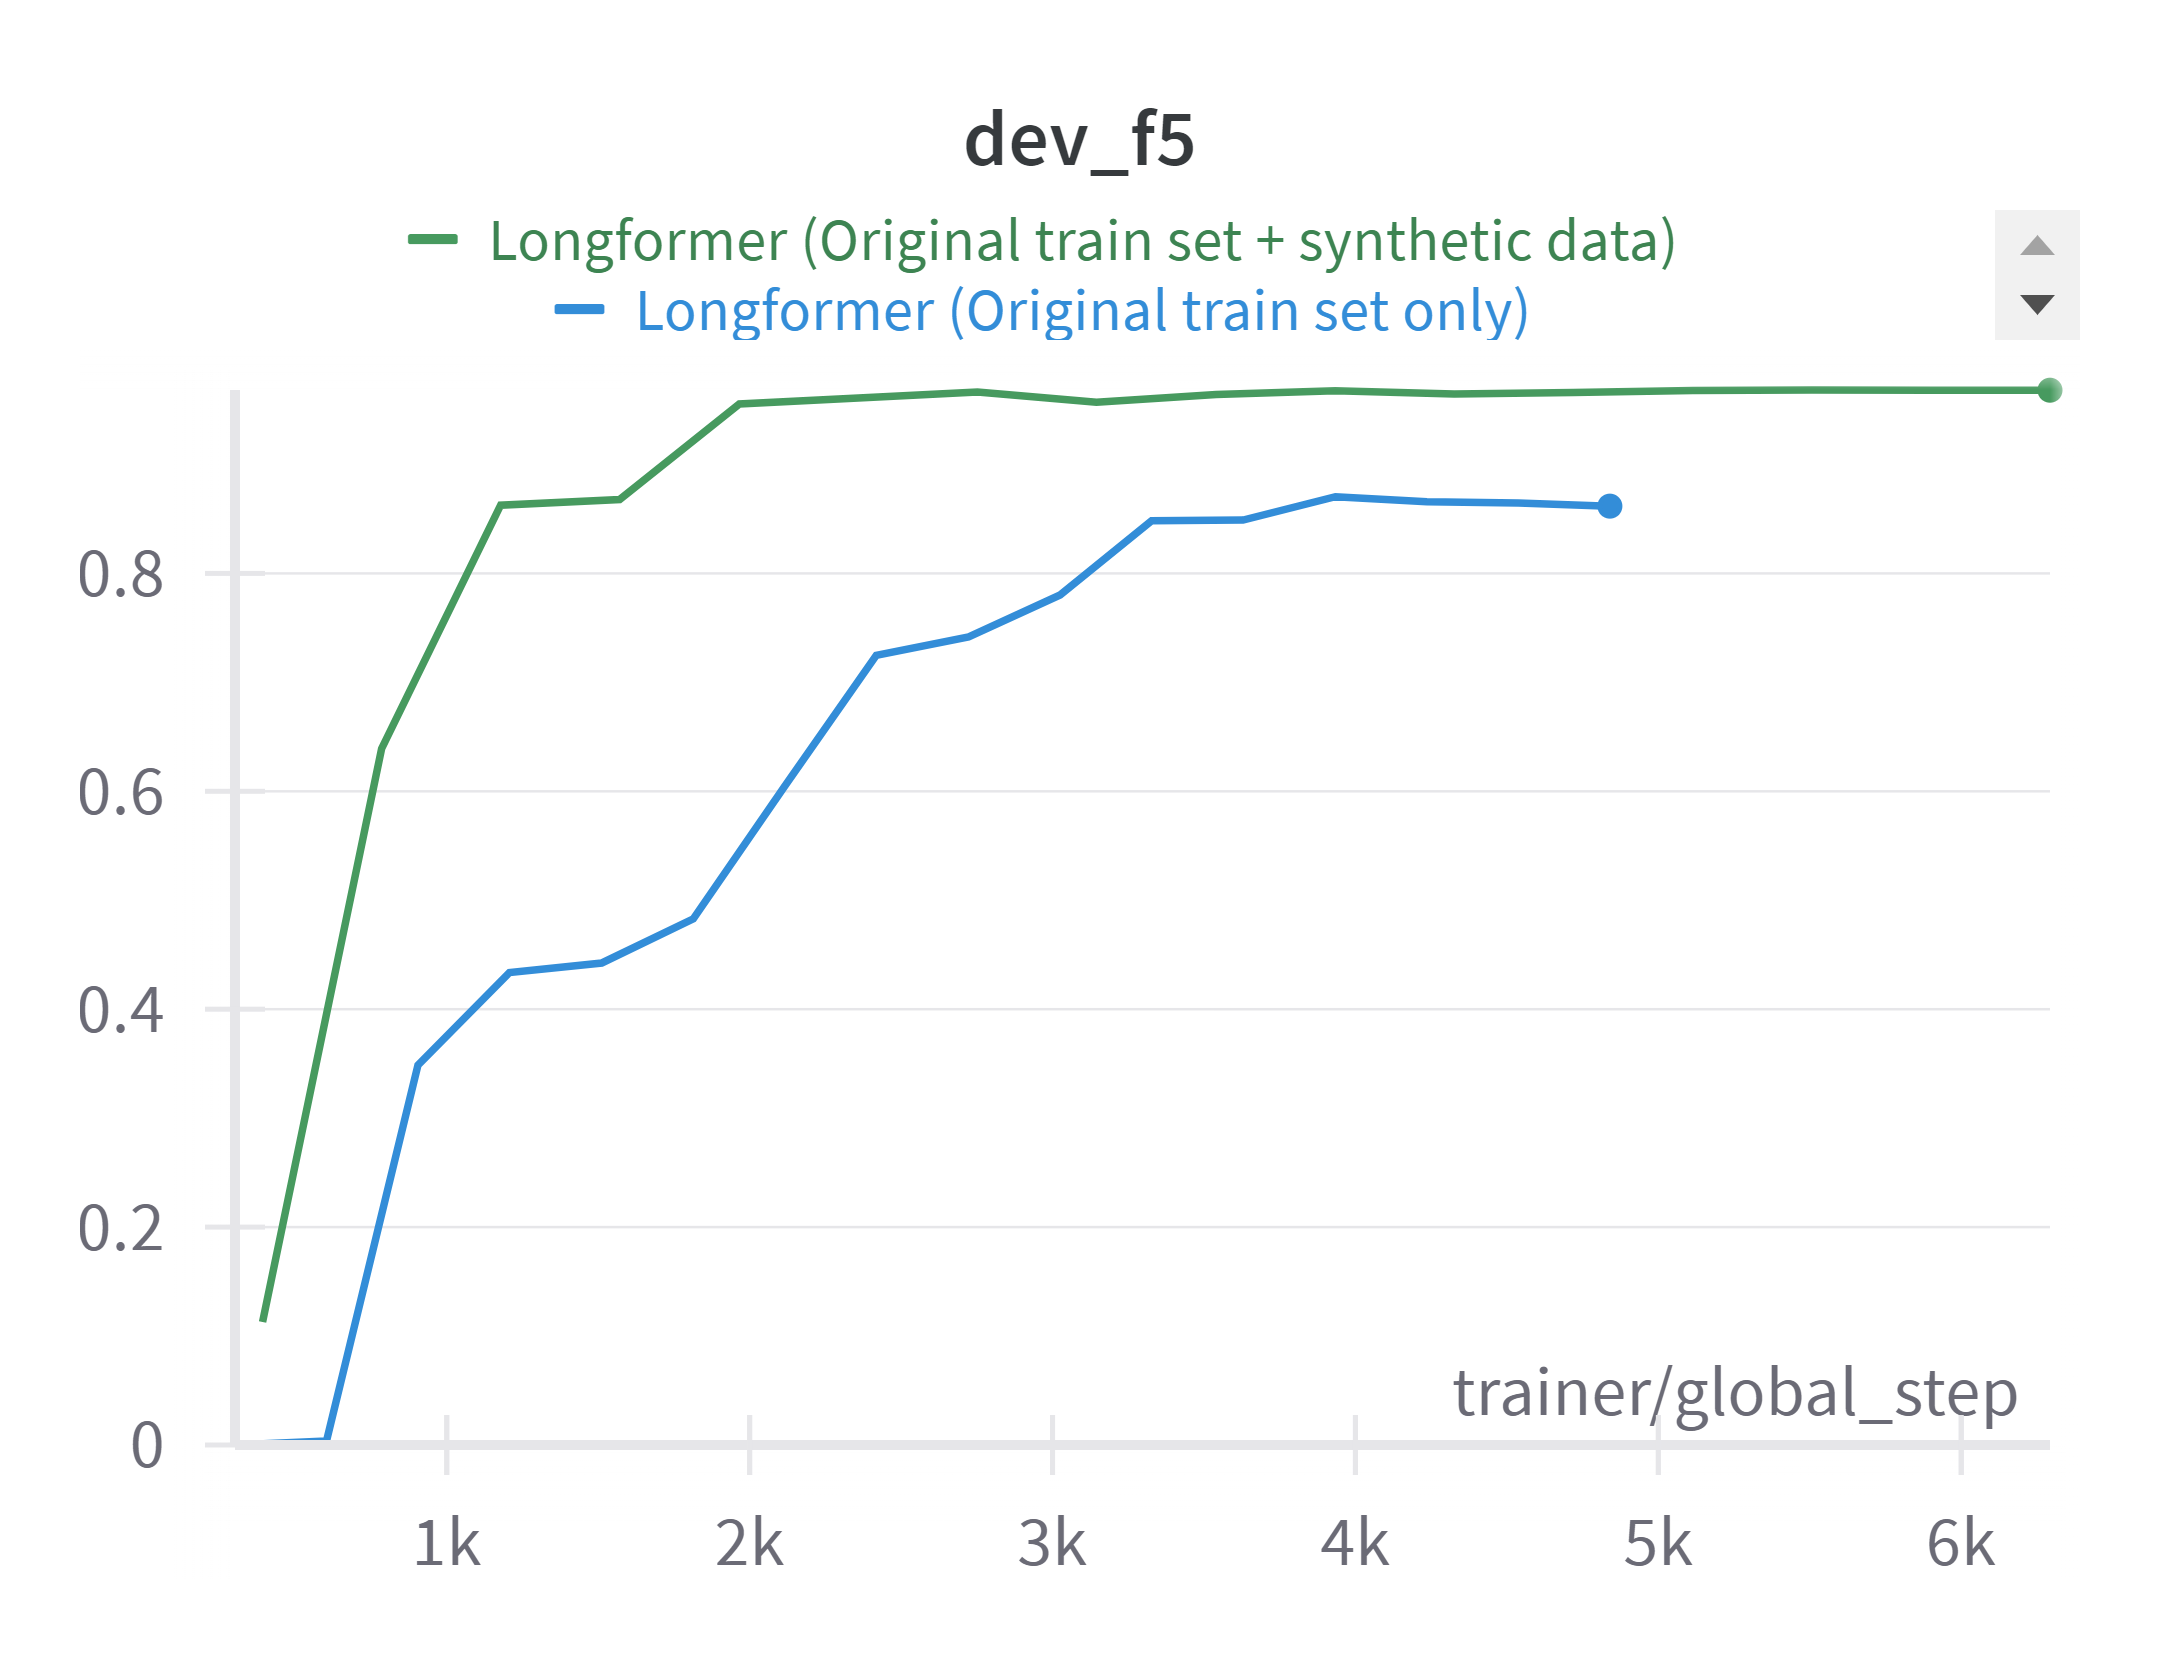
\includegraphics[width=\columnwidth]{images/dev_f5.png}
  \label{fig:dev_f5}
\end{figure}

\section{Methods}

\subsection{Benchmark: Presidio}

The benchmark is Presidio, a data protection and anonymization SDK developed by Microsoft. Presidio \cite{Presidio} consists of two main modules: a recognition engine and an anonymization engine. The recognition engine uses a combination of techniques to detect PII entities: regular expressions, NER using spaCy, and predefined context words. (I'm only interested in the recognition engine for the benchmark.)

Presidio was configured with its default settings. As per one of the benchmarks used in \citealt{pilan-etal-2022-text}, organization names are excluded to maintain a focus on \textit{personal} information. Considerations for adapting Presidio to the test set for my experiments:

\begin{itemize}
  \item Map Presidio's PII entity types to the corresponding types in the test set (for example, \texttt{PERSON} to \texttt{NAME\_STUDENT}). See \Tablink{tab:entity_label_mapping} for full map.
  \item Handling multi-token entities and assigning appropriate BIO labels (\texttt{B-} for the first token, \texttt{I-} for subsequent tokens within the same entity).
  \item Addressing potential overlaps between different entity types (for example, ensuring that a URL is not labeled as an \texttt{EMAIL\_ADDRESS} if it is part of a larger \texttt{URL} entity).
\end{itemize}

\begin{table}[h!]
  \centering
  \caption{Map of Presidio entity types to full labels.}
  \label{tab:entity_label_mapping}
  \begin{tabular}{ccc}
    \toprule
    \textbf{Presidio entity} & \(\rightarrow\) & \textbf{Corresponding type} \\
    \midrule
    \texttt{PHONE\_NUMBER} & \(\rightarrow\) & \texttt{PHONE\_NUM} \\
    \texttt{PERSON} & \(\rightarrow\) & \texttt{NAME\_STUDENT} \\
    \texttt{URL} & \(\rightarrow\) & \texttt{URL\_PERSONAL} \\
    \texttt{EMAIL\_ADDRESS} & \(\rightarrow\) & \texttt{EMAIL} \\
    \texttt{US\_SSN} & \(\rightarrow\) & \texttt{ID\_NUM} \\
    \bottomrule
  \end{tabular}
\end{table}

\subsection{Inference on fine-tuned Longformer models}

\begin{table*}[t]
  \centering
  \caption{Model names and abbreviations.}
  \label{tab:model_specs}
  \begin{tabularx}{\textwidth}{Xcc}
    \toprule
    \textbf{Model name} & \textbf{Checkpoint size} & \textbf{Abbreviated name} \\
    \midrule
    Longformer (Original train set only) & 609.0MB & \texttt{Lf(O)} \\
    Longformer (Original train set + synthetic data) & 609.0MB & \texttt{Lf(O+S)} \\
    \bottomrule
  \end{tabularx}
\end{table*}

The maximum sequence length for inference is 4096.

If the probability of the \texttt{O} label is below a threshold of 0.85, the non-\texttt{O} BIO label with the highest probability is selected.

\daggerfootnotes
\section{Metrics}
\numericfootnotes

To comprehensively evaluate the performance of Presidio and my original Longformer models in identifying PII in the test set, I used standard classifier metrics: precision, recall, and a weighted F-score.\footnote{As discussed in \href{https://web.stanford.edu/class/cs224u/slides/cs224u-methods-2023-handout.pdf}{CS224U: NLP methods and metrics}}

Precision, in the context of this project, measures the proportion of correctly predicted positive PII BIO labels among all the BIO labels predicted by the model. It reflects the model's ability to avoid false positives—a higher precision indicates the model is more likely to be correct when it predicts a token as PII. Precision is calculated as:

\begin{equation*}
\text{Precision} = \frac{\text{True Positives}}{\text{True Positives} + \text{False Positives}}
\end{equation*}

Recall measures the proportion of correctly positive PII BIO labels among the true set of PII BIO labels. A high recall represents a low proportion of PII tokens left undetected by the model—indicating the degree of privacy protection. Recall is calculated as:

\begin{equation*}
\text{Recall} = \frac{\text{True Positives}}{\text{True Positives} + \text{False Negatives}}
\end{equation*}

To quantify the balance between privacy protection and data utility preservation, I used the $F_\beta$ score. $F_\beta$ is the standard weighted harmonic mean of precision and recall—$\beta$ is the parameter that controls the relative importance of recall over precision. The $F_\beta$ score is calculated as:

\begin{equation*}
F_\beta = (1 + \beta^2) \cdot \frac{\text{precision} \cdot \text{recall}}{(\beta^2 \cdot \text{precision}) + \text{recall}}
\end{equation*}
 
I used $\beta=5$. Setting $\beta$ to 5 assigns five times more importance to recall over precision, reflecting the precedence of privacy protection over data preservation in the context of strict data anonymization requirements.\footnote{The \href{https://www.kaggle.com/competitions/pii-detection-removal-from-educational-data/leaderboard}{Kaggle leaderboard} for the competition uses this metric, so in case I want to submit my original model to the competition, it will be scored according to it.} 

I compute the precision, recall, and $F_5$ score for each PII type (see \hyperref[par:pii_types]{full list}) as well as the micro-averaged scores across all entity types. The micro-averaged scores assess the model's overall performance, considering the dataset as a single large document.

\section{Results} 

The top-line results are in \Tablink{tab:f5_values}.

\begin{table}[h!]
  \centering
  \caption{$F_5$ values for different models.}
  \label{tab:f5_values}
  \begin{tabular}{lr}
  \toprule
  \textbf{Model} & \textbf{$F_5$} \\
  \midrule
  Presidio & 0.735 \\
  \texttt{Lf(O)} & 0.831 \\
  \texttt{Lf(O+S)} & \textbf{0.936} \\
  \bottomrule
  \end{tabular}
\end{table}

See \Tablink{tab:precision_recall_f5} for granular results. 

\begin{table*}[t]
  \centering
  \caption{Precision ($P$), Recall ($R$), and $F_5$ values for different categories and models.}
  \label{tab:precision_recall_f5}
  \begin{tabularx}{\textwidth}{Xccccccccc}
    \toprule
    \textbf{PII type} & \multicolumn{3}{c}{Presidio} & \multicolumn{3}{c}{\texttt{Lf(O)}} & \multicolumn{3}{c}{\texttt{Lf(O+S)}} \\
    \cmidrule(lr){2-4} \cmidrule(lr){5-7} \cmidrule(lr){8-10}
    & $P$ & $R$ & $F_5$ & $P$ & $R$ & $F_5$ & $P$ & $R$ & $F_5$ \\
    \midrule
    \texttt{NAME\_STUDENT}     & 0.190 & 0.918 & 0.800 & 0.691 & 0.905 & 0.894 & 0.745 & 0.970 & \textbf{0.959} \\
    \texttt{URL\_PERSONAL}     & 0.0444 & 1.000 & 0.547 & 0.333 & 1.000 & 0.929 & 0.480 & 1.000 & \textbf{0.960} \\
    \texttt{EMAIL}             & 0.750 & 1.000 & \textbf{0.987} & 0.000 & 0.000 & 0.000 & 0.667 & 0.667 & 0.667 \\
    \texttt{PHONE\_NUM}        & 0.250 & 1.000 & 0.897 & 0.000 & 0.000 & 0.000 & 1.000 & 1.000 & \textbf{1.000} \\
    \texttt{STREET\_ADDRESS}   & 0.000 & 0.000 & 0.000 & 0.000 & 0.000 & 0.000 & 1.000 & 0.909 & \textbf{0.912} \\
    \texttt{ID\_NUM}           & 0.000 & 0.000 & 0.000 & 1.000 & 0.375 & 0.384 & 0.333 & 0.500 & \textbf{0.491} \\
    \texttt{USERNAME}          & 0.000 & 0.000 & 0.000 & 0.000 & 0.000 & 0.000 & 0.000 & 0.000 & 0.000 \\
    \bottomrule
  \end{tabularx}
\end{table*}

\section{Analysis} 

\subsection{Core analysis}

The metrics in \Tablink{tab:f5_values} show that the \texttt{Lf(O+S)} model achieves the highest overall $F_5$ score of 0.936, substantially outperforming both the Presidio benchmark ($F_5 = 0.735$) and the \texttt{Lf(O)} model ($F_5 = 0.831$).

\hl{This validates the primary hypothesis that the benchmark [Presido] will be significantly outperformed, as measured by standard classifier metrics [$F_5$], by a custom model fine-tuned on the train set of a high-quality, human-annotated, domain-specific dataset [\texttt{Lf(O)}]}.

Looking at the category-level metrics in \Tablink{tab:precision_recall_f5} provides further insight. The \texttt{Lf(O+S)} model achieves near-perfect $F_5$ scores above 0.95 for the most common categories of PII in original train set \texttt{NAME\_STUDENT} and \texttt{URL\_PERSONAL}. We clearly see \( F_5(\texttt{Lf(O+S)}) > F_5(\texttt{Lf(O)}) \gg F_5(\text{Presidio}) \) for these catagories. \hl{This supports the secondary hypothesis that the primary hypothesis holds principally because of \textit{in-context} PII, which is highly domain-specific.} Simply put, the more examples of this \textit{in-context} PII category that are learned—either from the original test set or the synthetic data—the better the fine-tuned Longformer model performs.

Interestingly, Presidio achieves a near-perfect $F_5$ score of 0.987 for \texttt{EMAIL}. Presidio uses a regular expression to identify this PII type, which beats the pure machine learning approach.

\subsection{Improvements and further research}

\begin{itemize}
\item One of the most surprising and interesting results of the experiements was the utility of synthetic data for significantly bolstering the performance of the Longformer model, particularly for categories with very few examples in the original train set. For instance, the $F_5$ score for \texttt{PHONE\_NUM} improved from 0.000 in \texttt{Lf(O)} to 1.000 in \texttt{Lf(O+S)}. Even for categories with relatively abundant examples, such as \texttt{NAME\_STUDENT}, the $F_5$ score increased by 0.065 with the addition of synthetic data. These findings suggest that the performance of the PII detection model could be further improved by conducting a more in-depth analysis of the train set structure and adopting a more systematic approach to generating fake PII sets and essay generation prompts. It would be interesting to explore the extent to which the original train set could be replaced by generated synthetic data without compromising the model's performance.
\item To enhance the model's performance on categories with limited examples, such as \texttt{ID\_NUM} and \texttt{USERNAME}, a fine-grained analysis of the existing examples in the train set should be conducted.
\item For real-world PII detection pipelines, a hybrid approach that combines the strengths of rule-based mechanisms, such as those employed by Presidio, with the fine-tuned Longformer model could yield promising results. Rule-based techniques can efficiently capture well-defined patterns and formats, while the Longformer model excels at understanding the nuanced context and identifying PII that may not adhere to strict rules. By leveraging the complementary strengths of these two approaches, a more comprehensive and robust PII detection system could be developed. 
\item To strengthen the Presidio benchmark, future work could explore extending its default recognizers with custom ones tailored to specific contexts, as demonstrated by \citealt{AzizStraiton2023PIIDetection} in their work on identifying Australian-specific PII types. In the context of this project, custom recognizers could be developed to better capture PII patterns specific to the educational domain or the United States, such as student ID formats, school-related abbreviations, or state-specific information. By incorporating these domain-specific recognizers, the Presidio benchmark would become a more challenging and relevant baseline for evaluating the performance of the Longformer model.
\end{itemize}

\section*{Known project limitations}

\begin{itemize}
\item The corpus comprises essays submitted in the context of a MOOC hosted by a university in the United States. We can assume most students are based in the United States. This means the models may not generalize well to identifying PII with local context outside the United States, such as identifying non-US phone number formats, addresses, or region-specific identification numbers.
\item The performance of the models may be sensitive to variations in PII formats or representations. For example, if a student writes their phone number in an unconventional way ("five-five-five, one-two-three, four-five-six-seven"), the model might not recognize it as a phone number. Robustness to such variations is an important consideration for practical applications.
\item The performance of the models on multilingual essays or essays containing non-English PII has not been evaluated.
\end{itemize}

\section*{Authorship statement}

This final project report was produced using the \href{https://www.overleaf.com/project/6237af8bd773a40c9da88358}{$LaTeX$ template} c/o Christopher Potts.

This was an individual project for a Stanford Center for Professional Development course (XCS224U) and there were no external contributors, reviewers or editors.

\bibliography{anthology,custom}

\end{document}
